% Study workflow. Build: tectonic workflow.tex
\documentclass[tikz,border=3pt]{standalone}
\usepackage[T1]{fontenc}
\usepackage{tgheros}
\renewcommand{\familydefault}{\sfdefault}
\usepackage{amsmath,amssymb}
\usepackage{sansmath}\sansmath
\usepackage{pifont}
\usetikzlibrary{arrows.meta,positioning,calc,shapes.geometric,fit,backgrounds}

% panel colours (frame / fill / title)
\definecolor{p1}{RGB}{196,82,120}  \definecolor{p1f}{RGB}{250,232,238}
\definecolor{p2}{RGB}{184,110,40}  \definecolor{p2f}{RGB}{252,240,224}
\definecolor{p3}{RGB}{48,128,72}   \definecolor{p3f}{RGB}{230,243,232}
\definecolor{p4}{RGB}{96,100,110}  \definecolor{p4f}{RGB}{238,239,242}
\definecolor{p5}{RGB}{110,84,170}  \definecolor{p5f}{RGB}{238,233,248}
\definecolor{p6}{RGB}{44,96,160}   \definecolor{p6f}{RGB}{228,238,250}
\definecolor{p7}{RGB}{196,96,40}   \definecolor{p7f}{RGB}{251,234,222}
% data colours
\definecolor{cB}{RGB}{74,120,168}  \definecolor{cBl}{RGB}{164,190,218} \definecolor{cBll}{RGB}{214,226,239}
\definecolor{cO}{RGB}{232,180,72}  \definecolor{cOl}{RGB}{244,214,150}
\definecolor{cG}{RGB}{88,160,104}  \definecolor{cGl}{RGB}{160,205,170}
\definecolor{cR}{RGB}{200,60,70}
\definecolor{d1}{RGB}{47,93,138} \definecolor{d2}{RGB}{233,128,40} \definecolor{d3}{RGB}{80,160,80}
\definecolor{d4}{RGB}{176,120,160} \definecolor{d5}{RGB}{110,180,170} \definecolor{d6}{RGB}{236,200,60}
\definecolor{d7}{RGB}{150,110,80} \definecolor{d8}{RGB}{185,180,175}

\tikzset{
  panel/.style={draw=#1,fill=#1f,line width=0.9pt,rounded corners=6pt},
  ptitle/.style={font=\bfseries\normalsize,text=#1,anchor=west},
  num/.style={circle,fill=#1,text=white,font=\bfseries\small,inner sep=0pt,minimum size=13pt},
  capt/.style={font=\scriptsize,align=center,text=black!85},
  small/.style={font=\tiny,align=center,text=black!80},
  arr/.style={-{Stealth[length=5pt]},line width=0.9pt,black!75},
  bigarr/.style={-{Stealth[length=7pt,width=7pt]},line width=1.8pt,black!80},
  chip/.style={draw=#1,fill=white,rounded corners=2pt,font=\tiny,inner sep=2pt,align=center,line width=0.6pt},
  sq/.style={minimum size=6.5pt,inner sep=0pt,draw=white,line width=0.4pt},
  tree/.pic={\begin{scope}[scale=0.78]
    \fill[black!80] (0,0) circle (2.2pt);
    \draw[black!60,line width=0.6pt] (0,0) -- (-0.32,-0.38) (0,0) -- (0.32,-0.38)
       (-0.32,-0.38) -- (-0.48,-0.74) (-0.32,-0.38) -- (-0.16,-0.74) (0.32,-0.38) -- (0.16,-0.74) (0.32,-0.38) -- (0.48,-0.74);
    \fill[black!55] (-0.32,-0.38) circle (1.8pt) (0.32,-0.38) circle (1.8pt);
    \foreach \x in {-0.48,-0.16,0.16,0.48} \fill[cG] (\x,-0.74) circle (1.8pt);
  \end{scope}},
}

\newcommand{\panel}[6]{% name, colour, x0, y0, x1, y1
  \draw[panel=#2] (#3,#4) rectangle (#5,#6);}
\newcommand{\ptitle}[5]{% colour, number, x, y, text
  \node[num=#1] at (#3,#4) {#2};
  \node[ptitle=#1] at ($(#3,#4)+(0.25,0)$) {#5};}

\begin{document}
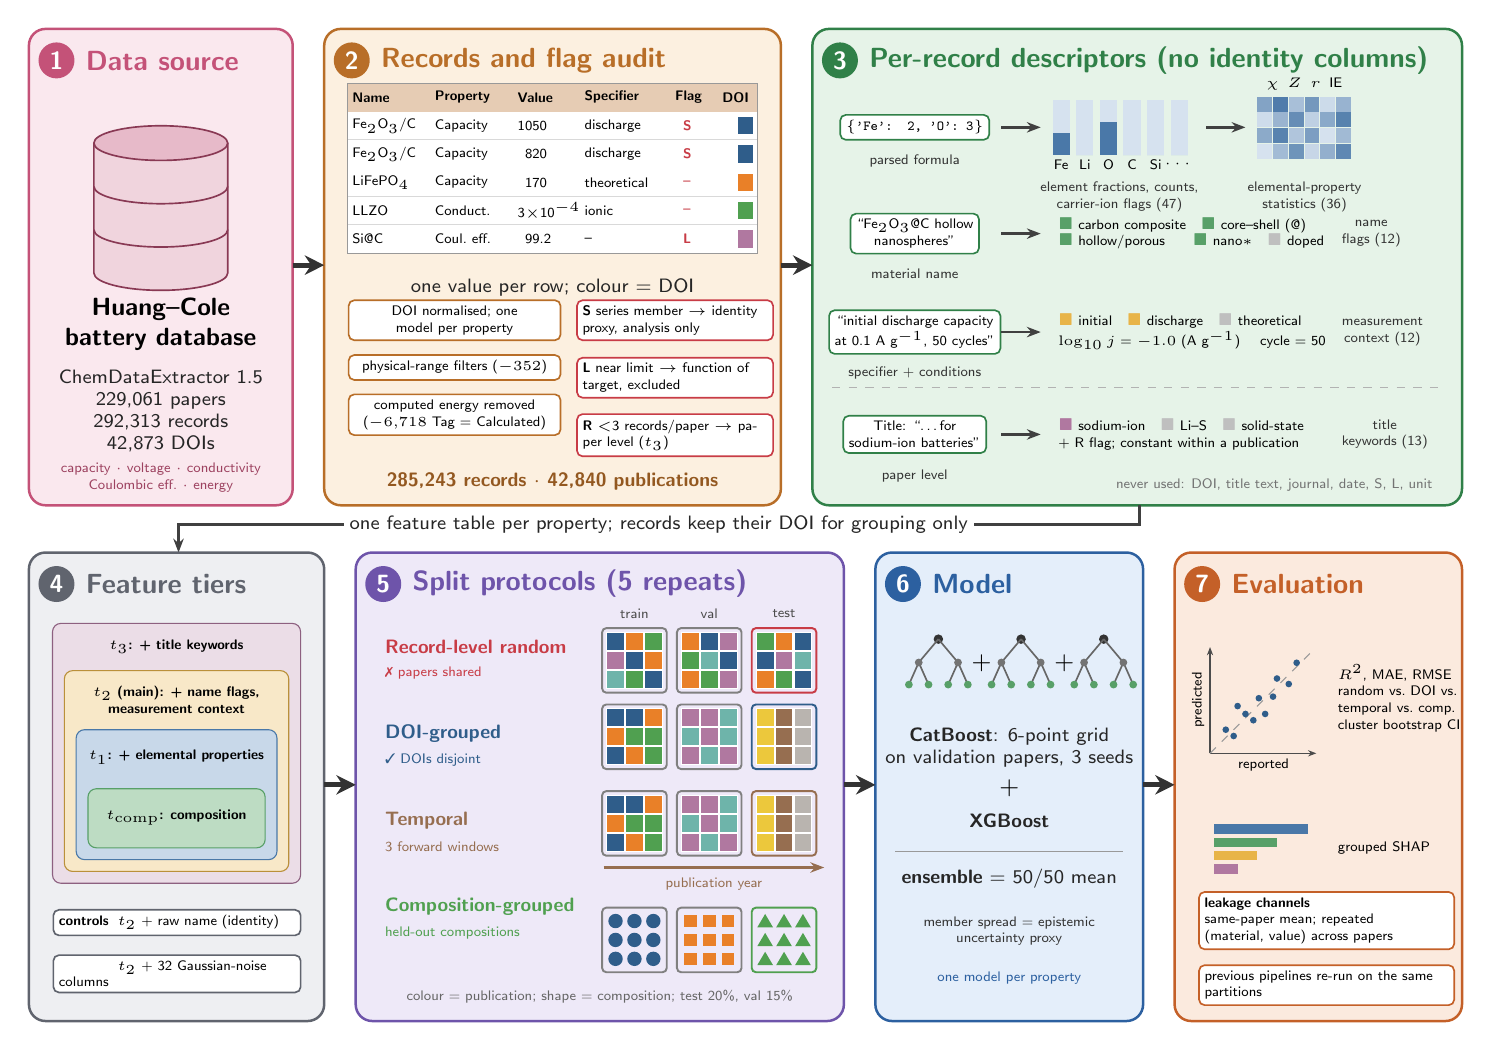
\begin{tikzpicture}[x=1cm,y=1cm]

% =============================================================== row 1
% ---------- 1 data source
\panel{a}{p1}{0}{6.55}{3.35}{12.6}
\ptitle{p1}{1}{0.35}{12.2}{Data source}
\begin{scope}[shift={(1.675,10.35)}]
  \foreach \yy in {-0.85,-0.3,0.25} {
    \fill[p1!25] (-0.85,\yy) rectangle (0.85,\yy+0.55);
    \fill[p1!25] (0,\yy) ellipse (0.85 and 0.22);
    \draw[p1!70!black,line width=0.6pt] (-0.85,\yy+0.55) -- (-0.85,\yy) arc (180:360:0.85 and 0.22) -- (0.85,\yy+0.55);}
  \fill[p1!40] (0,0.8) ellipse (0.85 and 0.22); \draw[p1!70!black,line width=0.6pt] (0,0.8) ellipse (0.85 and 0.22);
\end{scope}
\node[font=\bfseries\small,align=center] at (1.675,8.85) {Huang--Cole\\battery database};
\node[capt] at (1.675,7.75) {ChemDataExtractor 1.5\\229,061 papers\\292,313 records\\42,873 DOIs};
\node[small,text=p1!80!black] at (1.675,6.9) {capacity $\cdot$ voltage $\cdot$ conductivity\\Coulombic eff.\ $\cdot$ energy};

% ---------- 2 cleaning and flag audit
\panel{b}{p2}{3.75}{6.55}{9.55}{12.6}
\ptitle{p2}{2}{4.1}{12.2}{Records and flag audit}
% mini long-format table
\begin{scope}[shift={(4.05,11.55)}]
  \def\rh{0.36}
  \fill[p2!35] (0,0) rectangle (5.2,\rh);
  \foreach \x/\t in {0.05/Name,1.1/Property,2.15/Value,3.0/Specifier,4.15/Flag,4.75/DOI}
    \node[font=\tiny\bfseries,anchor=west,inner sep=0pt] at (\x,\rh/2) {\t};
  \foreach \i/\n/\p/\v/\s/\w/\c in {1/{Fe$_2$O$_3$\slash C}/Capacity/1050/discharge/S/d1,
                                   2/{Fe$_2$O$_3$\slash C}/Capacity/\phantom{1}820/discharge/S/d1,
                                   3/LiFePO$_4$/Capacity/\phantom{1}170/theoretical/--/d2,
                                   4/LLZO/Conduct./3$\times$10$^{-4}$/ionic/--/d3,
                                   5/Si@C/Coul.\ eff./\phantom{1}99.2/--/L/d4}{
    \fill[white] (0,-\i*\rh) rectangle (5.2,-\i*\rh+\rh);
    \draw[black!15] (0,-\i*\rh) -- (5.2,-\i*\rh);
    \node[font=\tiny,anchor=west,inner sep=0pt] at (0.05,-\i*\rh+\rh/2) {\n};
    \node[font=\tiny,anchor=west,inner sep=0pt] at (1.1,-\i*\rh+\rh/2) {\p};
    \node[font=\tiny,anchor=west,inner sep=0pt] at (2.15,-\i*\rh+\rh/2) {\v};
    \node[font=\tiny,anchor=west,inner sep=0pt] at (3.0,-\i*\rh+\rh/2) {\s};
    \node[font=\tiny\bfseries,anchor=west,inner sep=0pt,text=cR] at (4.25,-\i*\rh+\rh/2) {\w};
    \fill[\c] (4.95,-\i*\rh+0.07) rectangle (5.15,-\i*\rh+\rh-0.07);}
  \draw[black!40] (0,-5*\rh) rectangle (5.2,\rh);
\end{scope}
\node[capt,anchor=north] at (6.65,9.55) {one value per row; colour = DOI};
% cleaning chips
\node[chip=p2,anchor=west,text width=2.55cm] (c1) at (4.05,8.9) {DOI normalised; one model per property};
\node[chip=p2,anchor=west,text width=2.55cm] (c2) at (4.05,8.3) {physical-range filters ($-352$)};
\node[chip=p2,anchor=west,text width=2.55cm] (c3) at (4.05,7.7) {computed energy removed\\($-6{,}718$ Tag = Calculated)};
% flags
\node[chip=cR,anchor=west,text width=2.35cm,align=left] (f1) at (6.95,8.9) {\textbf{S} series member $\rightarrow$ identity proxy, analysis only};
\node[chip=cR,anchor=west,text width=2.35cm,align=left] (f2) at (6.95,8.17) {\textbf{L} near limit $\rightarrow$ function of target, excluded};
\node[chip=cR,anchor=west,text width=2.35cm,align=left] (f3) at (6.95,7.44) {\textbf{R} $<$3 records/paper $\rightarrow$ paper level ($t_3$)};
\node[font=\bfseries\scriptsize,text=p2!80!black] at (6.65,6.85) {285,243 records $\cdot$ 42,840 publications};

% ---------- 3 descriptors
\panel{c}{p3}{9.95}{6.55}{18.2}{12.6}
\ptitle{p3}{3}{10.3}{12.2}{Per-record descriptors (no identity columns)}
% row: composition
\node[chip=p3,font=\tiny\ttfamily] (in1) at (11.25,11.35) {\{'Fe': 2, 'O': 3\}};
\node[small,anchor=north] at (11.25,11.12) {parsed formula};
\draw[arr] (12.35,11.35) -- (12.85,11.35);
\begin{scope}[shift={(13.0,11.0)}]
  \foreach \e/\f/\c in {0/0.4/cB,1/0.0/cBl,2/0.6/cB,3/0.0/cBl,4/0.0/cBl,5/0.0/cBl}
    {\fill[cBll] (\e*0.3,0) rectangle (\e*0.3+0.22,0.7); \fill[\c] (\e*0.3,0) rectangle (\e*0.3+0.22,0.7*\f);}
  \foreach \e/\l in {0/Fe,1/Li,2/O,3/C,4/Si,5/$\cdots$} \node[font=\tiny] at (\e*0.3+0.11,-0.12) {\l};
\end{scope}
\node[small,anchor=north] at (13.85,10.78) {element fractions, counts,\\carrier-ion flags (47)};
\draw[arr] (14.95,11.35) -- (15.45,11.35);
\begin{scope}[shift={(15.6,10.95)}]
  \foreach \i in {0,...,5} \foreach \j in {0,...,3} {
    \pgfmathsetmacro{\v}{mod(\i*37+\j*53,100)}
    \fill[cB!\v!cBll] (\i*0.2,\j*0.2) rectangle (\i*0.2+0.19,\j*0.2+0.19);}
  \node[font=\tiny] at (0.6,0.95) {$\chi$ \;$Z$\; $r$ \;IE};
\end{scope}
\node[small,anchor=north] at (16.2,10.78) {elemental-property\\statistics (36)};
% row: name text
\node[chip=p3,font=\tiny] (in2) at (11.25,10.0) {``Fe$_2$O$_3$@C hollow\\nanospheres''};
\node[small,anchor=north] at (11.25,9.68) {material name};
\draw[arr] (12.35,10.0) -- (12.85,10.0);
\node[font=\tiny,align=left,anchor=west] at (12.95,10.0) {\textcolor{cG}{$\blacksquare$} carbon composite\quad \textcolor{cG}{$\blacksquare$} core--shell (@)\\\textcolor{cG}{$\blacksquare$} hollow/porous\quad\;\; \textcolor{cG}{$\blacksquare$} nano$\ast$\quad \textcolor{black!25}{$\blacksquare$} doped};
\node[small,anchor=west] at (16.55,10.0) {name\\flags (12)};
% row: measurement context
\node[chip=p3,font=\tiny] (in3) at (11.25,8.75) {``initial discharge capacity\\at 0.1 A g$^{-1}$, 50 cycles''};
\node[small,anchor=north] at (11.25,8.43) {specifier + conditions};
\draw[arr] (12.35,8.75) -- (12.85,8.75);
\node[font=\tiny,align=left,anchor=west] at (12.95,8.75) {\textcolor{cO}{$\blacksquare$} initial\quad \textcolor{cO}{$\blacksquare$} discharge\quad \textcolor{black!25}{$\blacksquare$} theoretical\\$\log_{10} j$ = $-1.0$ (A g$^{-1}$) \quad cycle = 50};
\node[small,anchor=west] at (16.55,8.75) {measurement\\context (12)};
% row: title keywords
\node[chip=p3,font=\tiny] (in4) at (11.25,7.45) {Title: ``\dots for\\sodium-ion batteries''};
\node[small,anchor=north] at (11.25,7.13) {paper level};
\draw[arr] (12.35,7.45) -- (12.85,7.45);
\node[font=\tiny,align=left,anchor=west] at (12.95,7.45) {\textcolor{d4}{$\blacksquare$} sodium-ion\quad \textcolor{black!25}{$\blacksquare$} Li--S\quad \textcolor{black!25}{$\blacksquare$} solid-state\\+ R flag; constant within a publication};
\node[small,anchor=west] at (16.55,7.45) {title\\keywords (13)};
\draw[black!30,dashed] (10.2,8.05) -- (17.95,8.05);
\node[small,anchor=south east,text=black!55] at (17.95,6.6) {never used: DOI, title text, journal, date, S, L, unit};

% connectors row 1
\draw[bigarr] (3.35,9.6) -- (3.75,9.6);
\draw[bigarr] (9.55,9.6) -- (9.95,9.6);

% =============================================================== row 2
\draw[arr,line width=1.1pt] (14.1,6.55) -- (14.1,6.3) -- (1.9,6.3) -- (1.9,5.95);
\node[capt,fill=white,inner sep=2pt] at (8.0,6.3) {one feature table per property; records keep their DOI for grouping only};

% ---------- 4 feature tiers
\panel{d}{p4}{0}{0}{3.75}{5.95}
\ptitle{p4}{4}{0.35}{5.55}{Feature tiers}
\begin{scope}[shift={(0.3,1.75)}]
  \draw[fill=d4!25,draw=d4!80!black,rounded corners=3pt] (0,0) rectangle (3.15,3.3);
  \draw[fill=cO!30,draw=cO!80!black,rounded corners=3pt] (0.15,0.15) rectangle (3.0,2.7);
  \draw[fill=cBl!60,draw=cB,rounded corners=3pt] (0.3,0.3) rectangle (2.85,1.95);
  \draw[fill=cGl!70,draw=cG,rounded corners=3pt] (0.45,0.45) rectangle (2.7,1.2);
  \node[font=\tiny\bfseries] at (1.575,0.83) {$t_\mathrm{comp}$: composition};
  \node[font=\tiny\bfseries] at (1.575,1.6) {$t_1$: + elemental properties};
  \node[font=\tiny\bfseries,align=center] at (1.575,2.33) {$t_2$ (main): + name flags,\\measurement context};
  \node[font=\tiny\bfseries] at (1.575,3.0) {$t_3$: + title keywords};
\end{scope}
\node[chip=p4,anchor=west,text width=3.0cm,align=left] at (0.3,1.25) {\textbf{controls}\; $t_2$ + raw name (identity)};
\node[chip=p4,anchor=west,text width=3.0cm,align=left] at (0.3,0.6) {\phantom{\textbf{controls}}\; $t_2$ + 32 Gaussian-noise columns};

% ---------- 5 splits
\panel{e}{p5}{4.15}{0}{10.35}{5.95}
\ptitle{p5}{5}{4.5}{5.55}{Split protocols (5 repeats)}
\newcommand{\grid}[4]{% x, y, colour list (9), border colour
  \begin{scope}[shift={(#1,#2)}]
  \foreach \c [count=\k from 0] in {#3} {
    \pgfmathtruncatemacro{\r}{\k/3}\pgfmathtruncatemacro{\q}{mod(\k,3)}
    \node[sq,fill=\c] at (\q*0.24,-\r*0.24) {};}
  \draw[#4,line width=0.7pt,rounded corners=1.5pt] (-0.17,0.17) rectangle (0.65,-0.65);
  \end{scope}}
\foreach \y/\name/\col in {4.75/Record-level random/cR, 3.65/DOI-grouped/d1, 2.55/Temporal/d7, 1.45/Composition-grouped/d3}
  \node[font=\scriptsize\bfseries,text=\col,anchor=west] at (4.4,\y) {\name};
\foreach \x/\l in {7.69/train,8.64/val,9.59/test} \node[font=\tiny,text=black!70] at (\x,5.17) {\l};
% random: same papers everywhere
\grid{7.45}{4.82}{d1,d2,d3,d4,d1,d2,d5,d3,d1}{black!50}
\grid{8.4}{4.82}{d2,d1,d4,d3,d5,d1,d2,d3,d4}{black!50}
\grid{9.35}{4.82}{d3,d2,d1,d1,d4,d5,d2,d3,d1}{cR}
\node[small,text=cR,anchor=west] at (4.4,4.42) {\ding{55} papers shared};
% DOI-grouped
\grid{7.45}{3.85}{d1,d1,d2,d2,d3,d3,d1,d2,d3}{black!50}
\grid{8.4}{3.85}{d4,d4,d5,d5,d4,d5,d4,d5,d4}{black!50}
\grid{9.35}{3.85}{d6,d7,d8,d6,d7,d8,d6,d7,d8}{d1}
\node[small,text=d1,anchor=west] at (4.4,3.32) {\ding{51} DOIs disjoint};
% temporal
\grid{7.45}{2.75}{d1,d1,d2,d2,d3,d3,d1,d2,d3}{black!50}
\grid{8.4}{2.75}{d4,d4,d5,d5,d4,d5,d4,d5,d4}{black!50}
\grid{9.35}{2.75}{d6,d7,d8,d6,d7,d8,d6,d7,d8}{d7}
\draw[arr,d7] (7.3,1.95) -- (10.1,1.95) node[pos=0.5,below,font=\tiny,text=d7] {publication year};
\node[small,text=d7,anchor=west] at (4.4,2.22) {3 forward windows};
% composition-grouped (shapes = composition)
\begin{scope}[shift={(0,-0.1)}]
\foreach \gx/\cl/\shape in {7.45/black!50/0, 8.4/black!50/1, 9.35/d3/2}{
  \draw[\cl,line width=0.7pt,rounded corners=1.5pt] (\gx-0.17,1.37+0.17) rectangle (\gx+0.65,1.37-0.65);}
\foreach \k in {0,...,8}{\pgfmathtruncatemacro{\r}{\k/3}\pgfmathtruncatemacro{\q}{mod(\k,3)}
  \fill[d1] (7.45+\q*0.24,1.37-\r*0.24) circle (2.6pt);
  \fill[d2] (8.4+\q*0.24-0.08,1.37-\r*0.24-0.08) rectangle +(0.16,0.16);
  \fill[d3] (9.35+\q*0.24,1.37-\r*0.24+0.09) -- +(-0.1,-0.17) -- +(0.1,-0.17) -- cycle;}
\end{scope}
\node[small,text=d3,anchor=west] at (4.4,1.12) {held-out compositions};
\node[small,anchor=south,text=black!60] at (7.25,0.1) {colour = publication; shape = composition; test 20\%, val 15\%};

% ---------- 6 model
\panel{f}{p6}{10.75}{0}{14.15}{5.95}
\ptitle{p6}{6}{11.1}{5.55}{Model}
\pic at (11.55,4.85) {tree}; \node[font=\small] at (12.1,4.55) {+};
\pic at (12.6,4.85) {tree}; \node[font=\small] at (13.15,4.55) {+};
\pic at (13.65,4.85) {tree};
\node[capt,anchor=north] at (12.45,3.85) {\textbf{CatBoost}: 6-point grid\\on validation papers, 3 seeds};
\node[font=\small\bfseries] at (12.45,2.95) {$+$};
\node[capt,anchor=north] at (12.45,2.75) {\textbf{XGBoost}};
\draw[black!40] (11.0,2.15) -- (13.9,2.15);
\node[capt,anchor=north] at (12.45,2.05) {\textbf{ensemble} = 50/50 mean};
\node[small,anchor=north] at (12.45,1.45) {member spread = epistemic\\uncertainty proxy};
\node[small,anchor=north,text=p6] at (12.45,0.75) {one model per property};

% ---------- 7 evaluation
\panel{g}{p7}{14.55}{0}{18.2}{5.95}
\ptitle{p7}{7}{14.9}{5.55}{Evaluation}
\begin{scope}[shift={(15.0,3.4)}]
  \draw[-{Stealth[length=3pt]},black!70] (0,0) -- (1.35,0); \draw[-{Stealth[length=3pt]},black!70] (0,0) -- (0,1.35);
  \draw[black!40,dashed] (0,0) -- (1.3,1.3);
  \foreach \x/\y in {0.2/0.3,0.3/0.22,0.45/0.5,0.55/0.42,0.62/0.7,0.8/0.72,0.85/0.95,1.0/0.88,1.1/1.15,0.35/0.6,0.7/0.5}
    \fill[d1] (\x,\y) circle (1.2pt);
  \node[font=\tiny,rotate=90] at (-0.15,0.68) {predicted};
  \node[font=\tiny] at (0.68,-0.15) {reported};
\end{scope}
\node[font=\tiny,align=left,anchor=west] at (16.5,4.1) {$R^2$, MAE, RMSE\\random vs.\ DOI vs.\\temporal vs.\ comp.\\cluster bootstrap CI};
\begin{scope}[shift={(15.05,2.55)}]
  \foreach \w/\c [count=\i] in {1.2/cB,0.8/cG,0.55/cO,0.3/d4} \fill[\c] (0,-\i*0.17) rectangle (\w,-\i*0.17+0.12);
\end{scope}
\node[font=\tiny,align=left,anchor=west] at (16.5,2.2) {grouped SHAP};
\node[chip=p7,anchor=north west,text width=3.1cm,align=left] at (14.85,1.65) {\textbf{leakage channels}\\same-paper mean; repeated\\(material, value) across papers};
\node[chip=p7,anchor=north west,text width=3.1cm,align=left] at (14.85,0.72) {previous pipelines re-run on the same partitions};

% connectors row 2
\draw[bigarr] (3.75,3.0) -- (4.15,3.0);
\draw[bigarr] (10.35,3.0) -- (10.75,3.0);
\draw[bigarr] (14.15,3.0) -- (14.55,3.0);
\end{tikzpicture}
\end{document}
